\documentclass[a4paper,11pt]{article}
%\usepackage[T1]{fontenc}

%\setlength{\textwidth}{20cm}
%\setlength{\marginparwidth}{0cm}
%\setlength{\voffset}{0cm}
\usepackage[utf8]{inputenc}
\usepackage[francais]{babel}
\usepackage{amsmath}
\usepackage{graphicx}

%\special{papersize=210mm,297mm}

\title{{\Huge Electronique numérique}\\Logique séquentielle}
%\title{TD1}
\date{}

\begin{document}
\maketitle

{\it Tous les exercices ne seront pas forcément résolus en TE.}

% ANNEE prochaine ==> load avec registre à décallage


\section{Découverte de la bascule D}
Le symbole de la bascule D, ainsi que sa table de vérité sont rappelés ici.\\

\begin{figure}[!h]
\begin{center}
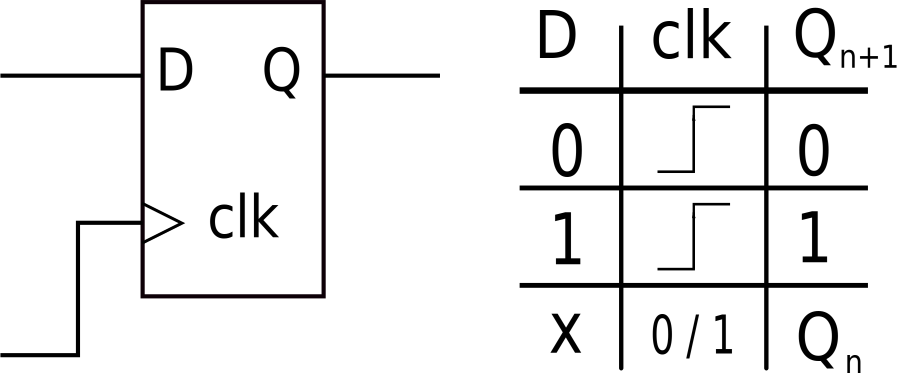
\includegraphics[scale=0.2]{./figures/d-ff-infos.jpg}
\end{center}
\end{figure}

La bascule D a pour fonction de recopier l'entrée D sur sa sortie Q, lors d'un court temps d'échantillonnage : il s'agit généralement du front montant de l'horloge. Cette horloge est supposée périodique. Pour que l'échantillonnage se passe correctement, le signal d'entrée doit respecter deux contraintes : il doit être parfaitement stable {\it avant} et {\it après} le front montant. Ces instants s'appellent temps de {\it setup} et temps de {\it hold}. La donnée est électriquement recopiée après un instant également très court appelé ``clock to Q''. Tous ces temps sont très inférieurs à la période d'horloge. {\bf La bascule D permet ainsi de travailler sur un signal stable, pendant toute une période} : le temps est désormais {\bf discrétisé}. Il n'y a plus à se soucier des temps de propagation caractéristiques -- et parfois fluctuants-- des différentes portes logiques réalisant les calculs ! Il suffit d'attendre une période d'horloge suffisamment longue pour observer un résultat combinatoire correct, échantillonné dans une bascule. L'écoulement du temps ne se fait que par 'quantum' de temps : celui des 'tops' (ou 'ticks') de cette horloge périodique. Il est même possible d'abstraire le fonctionnement du circuit encore plus en supposant que seuls ces instants d'échantillonnage sont significatifs et que les calculs s'effectuent instantanément sur ces 'tops' (on parle de calcul en ``temps zéro''), et que rien ne se passe entre ces 'tops' ! Mais cela reste 'une vue de l'esprit'.\\

Compléter le chronogramme suivant où un signal $S_1$ sur 4 bits, extérieur au système, est fourni comme entrée (sous sa forme entière).

\begin{figure}[!h]
\begin{center}
\includegraphics[scale=0.4]{./figures/dff-1.png}
\end{center}
\end{figure}


On précise ici que :
\begin{itemize}
\item nous ne tenons pas compte de la notion de temps de {\it setup} et temps de {\it hold}, ni du temps $t_{clk-2-Q}$
\item les zones de transistion des 4 bits se présentent ici comme des 'X'.
\item pour les signaux internes au système, on ne représentera pas ces transitions, supposées idéales : seuls des rectangles suffiront.
\item on suppose que les sorties Q sont initialisées à 0.
\end{itemize}


\section{Du circuit au chronogramme}

Soit le circuit logique suivant.

\begin{figure}[!h]
\begin{center}
\includegraphics[scale=0.3]{./figures/fsm-ex1.png}
\end{center}
\end{figure}

Sachant que la bascule D est initialisée à 0, trouver le chronogramme de la sortie $out$ correspondante, lorsque les valeurs d'entrée sont (respectivement, à chaque coup d'horloge) :

\begin{verbatim}
e1 : 0 1 0 1 1 0 1
e2 : 1 1 1 0 1 0 0
\end{verbatim}

\section{Du chronogramme au circuit}
Nous proposons ici un exercice plus rare, uniquement par jeu : il s'agit de retrouver le circuit qui a généré les chronogrammes suivants. Il y a probablement plusieurs solutions ! Soyez perspicaces ! Les signaux $e_i$ représentent des entrées, les signaux $s_i$ des sorties, et les signaux $n_i$ des signaux internes.

\begin{verbatim}
e1 : 0 0 1 1 0 0 0 0 1 1 0 0 1 0 0 0 0
e2 : 0 0 0 0 1 0 0 1 0 1 1 0 1 1 0 0 0
n1 : 0 0 1 1 1 0 0 1 1 1 1 0 1 1 0 0 0
s1 : 0 0 1 0 0 0 0 1 0 0 0 0 1 0 0 0 0
s2 : 1 1 0 1 1 1 1 0 1 1 1 1 0 1 1 1 1
s3 : ? 1 1 0 1 1 1 1 0 1 1 1 1 0 1 1 1
\end{verbatim}


% \section{Du circuit au diagramme à bulles}
% On reprend ici l'exercice 2. Notre but est désormais de trouver le diagramme états-transitions.
%
% En supposant que la bascule se trouve dans l'état 0 au démarrage du circuit, décrire le diagramme à bulle du système.\\

% {\bf solution : }
%
% Le circuit ne possède qu'une seule bascule D donc un seul bit d'état, ce qui va beaucoup nous aider. On écrit la table de vérité de la fonction de transition $f_{trans}(e_1,e_2,Q)$ :
%
% \begin{table}[H]
% \begin{center}
%     \begin{tabular}{|c|c|c||c||c|}
%         \hline
%         e1 & e2 & Q & D & ligne \\ \hline \hline
%         0  & 0  & 0 & 0 & 0 \\
%         0  & 0  & 1 & 0 & 1 \\
%         0  & 1  & 0 & 1 & 2 \\
%         0  & 1  & 1 & 1 & 3 \\
%         1  & 0  & 0 & 0 & 4 \\
%         1  & 0  & 1 & 1 & 5 \\
%         1  & 1  & 0 & 1 & 6 \\
%         1  & 1  & 1 & 1 & 7 \\
%         \hline
%     \end{tabular}
% \end{center}
% \end{table}
%
% Appelons E cette variable d'état. L'état courant de E est matérialisé par Q et sont état futur par D. Comment évolue cette variable au cours du temps ? On peut dessiner le diagramme à bulle suivant (ou diagramme d'état), et faire donc apparaître 4 conditions booléennes possibles, appelées $k_1,k_2,k_3,k_4$, relatives aux transitions. \\
%
% \begin{figure}[H]
% \begin{center}
% \includegraphics[scale=0.2]{./exo5.png}
% \end{center}
% \end{figure}
%
% Trouvons alors ces $k_1,k_2,k_3,k_4$ :\\
%
% \begin{itemize}
% \item E passe de 0 à 0 sur les lignes 0 et 4 d'où la condition $k_1=\overline{e_2}$
% \item E passe de 0 à 1 sur les lignes 2 et 6 d'où la condition $k_2=e_2$ (soit encore $k_2=\overline{k_1}$).
% \item E passe de 1 à 1 sur les lignes 3, 5 et 7 d'où la condition $k_3=e_1+e_2$
% \item E passe de 1 à 0 sur les lignes 1, d'où la condition $k_4=\overline{e_1}.\overline{e_2}$ (soit encore $k_4=\overline{k_3}$).
% \end{itemize}

\section{Suite de Fibonacci en circuit}
La suite de Fibonacci est bien connue : $u_{n+2}=u_{n+1}+u_{n}$, où $u_{1}=1$ et $u_0=0$.
Elle date de 1202 et décrit la croissance d'une population de lapins, à partir d'un seul couple.
Pour la petite histoire, cette suite a par ailleurs un lien étonnant avec le nombre d'or $\phi=\frac{1+\sqrt{5}}{2} \approx 1.628$.
En effet, Euler a démontré que pour un $n$ donné (un "step"), on a :
$$u_n=\frac{1}{\sqrt{5}}(\phi^n - \phi'^n) \textrm{ , où } \phi' = - \frac{1}{\phi}$$

\begin{enumerate}
  \item Dessiner le circuit numérique émettant la suite de Fibonacci. Un changement d'indice simple, au préalable, est conseillé.
  \item Chaque bascule D possède un reset actif haut, et un set actif bas. Compléter le schéma précédent, de manière à initialiser correctement les bascules. On dispose d'un bouton poussoir
  d'initialisation qui fournit un signal de {\it reset} actif {\it haut} : lorsqu'on appuie sur ce bouton pour initialiser le circuit, ce signal vaut '1'.
\end{enumerate}

\end{document}
